\subsubsection{Opcodes} \label{sec:implementation_opcodes}

Within the defined task for this work, there are several operations that the architecture must be able to execute:

\begin{itemize}
    \item Memory access (Load, Store, Move)
    \item Flow control ((Conditional) Jump)
    \item (Un-) signed addition
    \item (Un-) signed subtraction
    \item Bitwise operations (AND, OR, NOT)
    \item Bitwise shifting (Left and right) 
\end{itemize}

Each of these operations must be assigned its unique opcode so the control logic knows what operation to perform during a cycle. As discussed in \autoref{sec:implementation_isa_memory_model}, an operation can be emulated by using another operation. Therefore, the number of actual opcodes defined in an \ac{isa} may be smaller than the number of usable instructions within a programming language. However, there is no general way to substitute the fundamental arithmetic operations of addition, subtraction and bitwise shifting to the left or right. Therefore, these four operations receive one opcode each.


\begin{wrapfigure}{r}{0.5\textwidth}
    \centering
    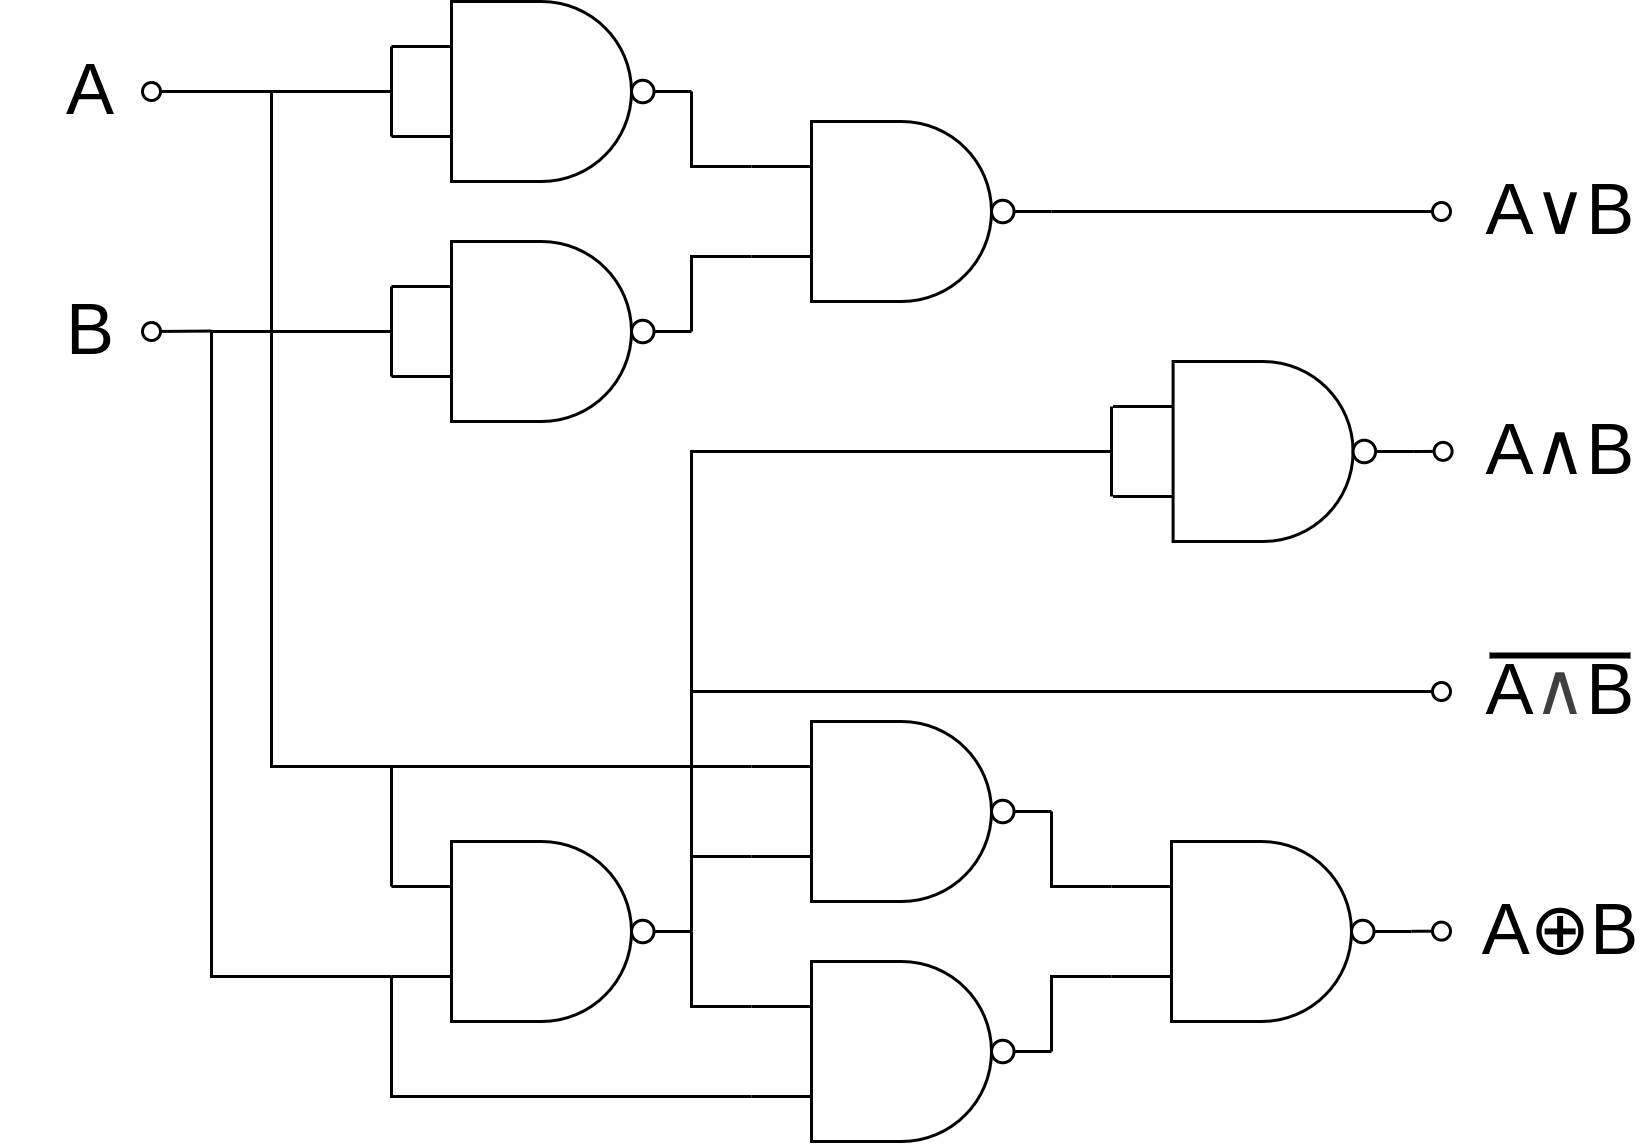
\includegraphics[width=0.48\textwidth]{images/drawio/bitwise_operators_logic.png}
    \caption{Logic gates implementing OR, AND, XOR, NAND while reusing intermediary results}
    \label{fig:logic_gates_binary_operators}
\end{wrapfigure}\leavevmode

In total, the \ac{alu} must be able to perform these seven different operations. However, it is a logically free-standing module and will likely be implemented as an individual piece of hardware, too. Therefore, the opcode or the relevant bits encoding the \ac{alu} operation must be passed to the implementing device as an individual piece of data. This piece of data requires $\lceil log_2(8) \rceil = 3$ bits to encode. Since there are only 7 required operations, one value represented by the 3 bits would not be assigned an operation. For this reason, the set of the three required bitwise operations \texttt{\{AND, OR, NOT\}} is replaced by \texttt{\{OR, AND, XOR, NAND\}}. As discussed in \autoref{sec:logical_operators}, this set is functionally complete, therefore any other set of boolean operators can be built from it. From the original required set of bitwise operations, \texttt{AND} and \texttt{OR} are retained, and \texttt{NOT} can be emulated by both the \texttt{XOR} and \texttt{NAND} operations. Since \texttt{NOT} is the only unary operator, emulating it by using the binary \texttt{NAND} simplifies an implementation since it also only needs to support binary operations.

This specific set of operators is chosen for the large amount of shared intermediary results of their boolean expression when built from \texttt{NAND} logic gates. Therefore, many of these results can be used for several of the operators. \autoref{align:binary_operators_from_nand} shows the boolean expressions, \autoref{fig:logic_gates_binary_operators} shows an efficient implementation of all operators using only 9 \texttt{NAND} gates.

\begin{align}
    A \lnand B &= A \lnand B \\
    A \land B  &= (A \lnand B) \lnand (A \lnand B) \\
    A \lor B   &= (A \lnand A) \lnand (B \lnand B) \\
    A \lxor B  &= (A \lnand (A \lnand B)) \lnand ((B \lnand (A \lnand B)))
\end{align}
\captionof{table}{Boolean expressions for binary operators OR, AND, XOR, NAND using only NAND operators}
\label{align:binary_operators_from_nand}
\vspace{\baselineskip}

However, this only defines the set of operations the \ac{alu} can perform by itself. It does not define the environment under which the \ac{alu} in invoked. For example, an arithmetic instruction may use operands from differen data sources such as registers, an immediate value encoded in the instruction or memory. From past experience, it also proves useful to have arithmetic instructions that do not modify the state of the flags register. An example of a use case for this is when implementing a stack in software. When pushing a value to this stack, the stack pointer must be incremented or decremented. If no addition can be performed without modifying the flags register, executing a \texttt{PUSH} instruction would therefore modify it as well. Therefore, early revisions of the AVA \ac{isa} defined a ``flags'' bit as part of the opcode that specified whether the flag output of the \ac{alu} shall update the flags register ``R5'' or not. 

Similarly, the 3 bit \ac{alu} opcode was a direct subsection of the general opcode. However, this resulted in multiple unrelated opcodes performing the same \ac{alu} operation. This in turn imposed implicit restrictions on the way the opcodes were assigned. Therefore, this was later changed and the \ac{alu} operation is selected using only control signals, which are assignable to arbitrary opcodes. In the current revision, the opcode is merely a number used to index into a table of control signals. This way, the assignment of operations to opcodes is fully arbitrary. No control signal depends on the opcode directly. This allows multiple different sets of instructions to be defined using the same hardware, provided the implementation allows updating the control signal table.

Instead, each arithmetic is assigned multiple instructions that have the following naming scheme:

\begin{table}[H]
    \centering
    \begin{tabular}{ll}
        XXX    & Perform the base instruction, using a register operand       \\
        XXXI   & Using an immediate operand                                   \\
        XXXNF  & Using a register operand, not updating the flags register    \\
        XXXINF & Using an immediate operand, not updating the flags register 
    \end{tabular}    
    \label{tab:instruction_suffices}
    \captionof{table}{Effect of instruction suffix on arithmetic instructions (XXX represents an arbitrary arithmetic operation)}
\end{table}

This increases the number of opcodes assigned to arithmetic operations four-fold, resulting in 32 opcodes for the 8 base operations. However, the added flexibility for laying out the opcode assignments is deemed worth the tradeoff.

\subsubsection{Types of Instruction}

The instructions of the AVA \ac{isa} largely fall into the three groups of computation, memory access and flow control. Since the opcodes are freely assigned, there is no way to determine the type of instruction from the opcode only. Also, since there is no control signal to disable the \ac{alu}, technically, all operations perform some computation, even if the result is discarded. Some computation operations also discard the result but retain the flags for future use, similar to comparison instructions in other architectures (i.e \texttt{cmp} in x86 \cite{intelASM86Manual1983}). In this work, any operation that modifies the state of one or more general purpose register is considered a computational one. Memory access operations are ones where the \ac{ram} is accessed, i.e the \texttt{LOAD} and \texttt{STORE} operations. Flow control operations are ones that potentially modify the program counter (depending on some condition).


\begin{table}[H]
    \centering
    \begin{tabular}{|c|c|c|c|l|} 
        \hline
        \textbf{Opcode} & \textbf{Name} & \textbf{Variants} & \textbf{Category} & \textbf{Description}             \\ 
        \hline
        0               & NOP           &                   & Flow Control      & No effects                       \\ 
        \hline
        1-4             & ADD           & I, NF, INF        & Arithmetic        & Add two numbers                  \\ 
        \hline
        5-8             & ADC           & I, NF, INF        & Arithmetic        & Add two numbers with carry       \\ 
        \hline
        9-12            & SUB           & I, NF, INF        & Arithmetic        & Subtract two numbers             \\ 
        \hline
        13-16           & SBC           & I, NF, INF        & Arithmetic        & Subtract two numbers with carry  \\ 
        \hline
        17-20           & SHL           & I, NF, INF        & Arithmetic        & Shift left                       \\ 
        \hline
        21-24           & SHR           & I, NF, INF        & Arithmetic        & Shift right                      \\ 
        \hline
        25-28           & OR            & I, NF, INF        & Arithmetic        & Bitwise logical OR               \\ 
        \hline
        29-32           & AND           & I, NF, INF        & Arithmetic        & Bitwise logical AND              \\ 
        \hline
        33-36           & XOR           & I, NF, INF        & Arithmetic        & Bitwise logical XOR              \\ 
        \hline
        37-40           & NAND          & I, NF, INF        & Arithmetic        & Bitwise logical NAND             \\ 
        \hline
        41-42           & LW            & I                 & Memory Access     & Load word                        \\ 
        \hline
        43-44           & SW            & I                 & Memory Access     & Store word                       \\ 
        \hline
        45-46           & BZ            & I                 & Memory Access     & Branch if zero                   \\ 
        \hline
        47-48           & BNZ           & I                 & Memory Access     & Branch if not zero               \\ 
        \hline
        49              & HCF           &                   & Flow Control      & Halt execution                   \\
        \hline
    \end{tabular}
    \label{tab:instructions}
    \captionof{table}{Supported instructions and their opcodes, variants, type and brief description (variant suffices are explained in \autoref{tab:instruction_suffices})}
\end{table}

At the time of writing, there are a total of 50 unique instructions, as well as 20 pseudo-instructions implemented within the assembler software. \autoref{tab:instructions} shows a listing of all instructions defined in the \ac{isa}.

\subsubsection{Instruction Encoding} \label{sec:implementation_instruction_encoding}

To simplify the implementation, all instructions use the same fixed length instruction encoding format. This way, one instruction word at a time is fetched from program memory, regardless of the instruction being read. An implementation can then directly route use the outputs of the program memory as the control signals without any further decoding logic. By doing so, the fetching circuitry can be implemented as a single, asynchronous unit. Since the architecture follows a strict Harvard architecture, the program memory is fully decoupled from the working memory. Therefore, the length of the instruction encoding can be chosen freely. After initial experimentation with 16 bit encodings, this was deemed too restrictive to implement a usable, practical \ac{isa}. The current revision uses a 32 bit word per instruction. \autoref{fig:ava_instruction_encoding} shows the fixed length instruction encoding format used in the AVA \ac{isa}.

\begin{figure}[H]
    \centering
    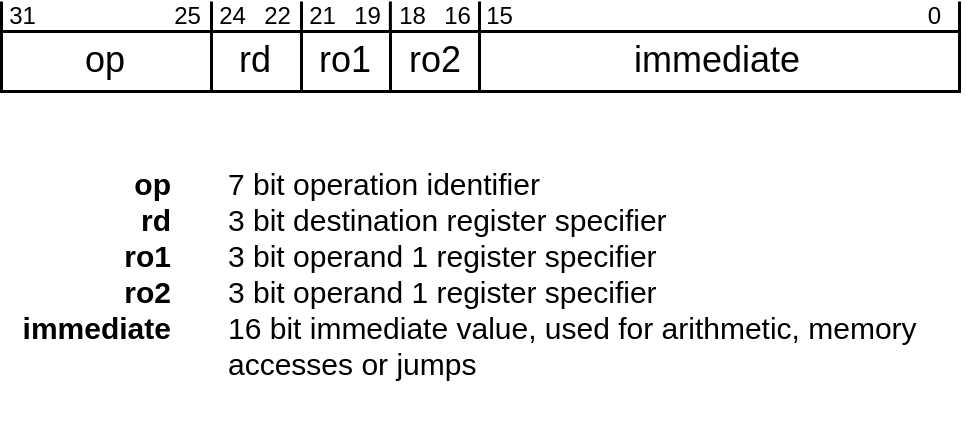
\includegraphics[width=0.7\textwidth]{images/drawio/ava_instruction_encoding.png}  % Replace with your image file
    \caption{AVA 32 bit instruction encoding scheme and field descriptions. Numbers above fields represent bit positions within the instruction}
    \label{fig:ava_instruction_encoding}
\end{figure}